
I want to find the Coincident Economic Index with more recent data. Then, I take US data from Refinitiv on Industrial Production (USIPMANG), total disposable personal incomes (USGPYD), total machinery manufacturing (USPPM), and weekley average work hous in nonfarm payrolls (USWRKW).  I am taking data from 2007:01-2012:12.


\begin{figure}[h!]
	\centering
	\captionsetup{width=0.5\textwidth, font=small}
	\caption{$C_{t|t}$ together with a 5\% confidence interval (assuming gaussianity) using data from 2007:01 to 2022:12.}\label{fig:new_cei}
	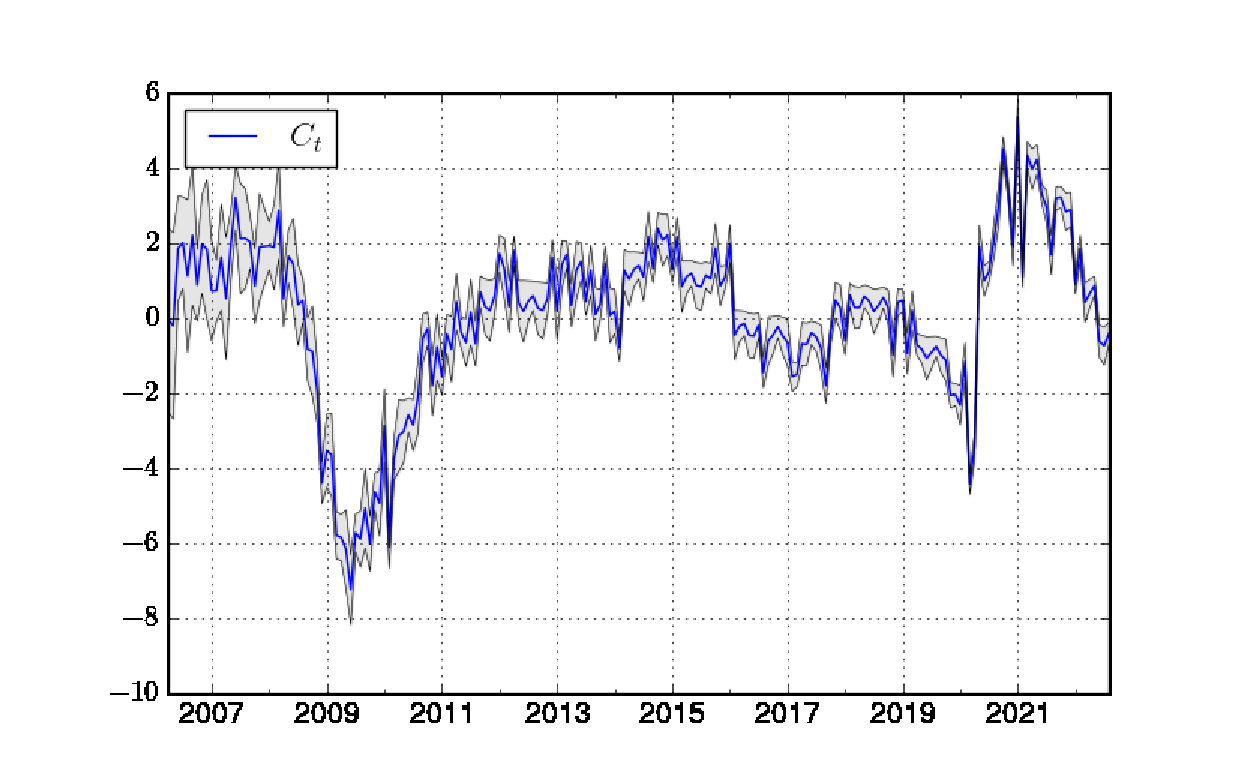
\includegraphics[scale=0.5]{fig/newdata_CEI}
\end{figure}

% employees on non agricultural payrolls.
\subsection{Preliminary analysis}

I repeat the same analysis: I check whether the series are integrated and, if they are, whether they are cointegrated.  For each of the the coincident indicators, \citeA{dickey1979distribution} test for a unit root (against the alternative that the series are stationary, perhaps around a linear time trend) was unable to reject (at the 10\% level) the hypothesis that the series are integrated. P-values are reported in Table \ref{tab:new_df_pvalues}.

\begin{table}[h!]
	\centering\small
	\captionsetup{width=0.6\textwidth, font=small}
	\caption{P-values of the test \protect\citeA{dickey1979distribution} for a unit root applied to the four series used in the index estimation. We fail to reject in every case at thte 10\%.}\label{tab:new_df_pvalues}
	\vspace{0cm}
	\begin{tabular}{l|rrrr}

{} & USIPMANG & USGPYD & USPPM & USWRKW \\ \hline\hline

p value &     0.08 &   0.91 &  0.98 &   0.47 \\ \hline\hline

\end{tabular}

\end{table}

The subsequent aplication of the \citeA{engle1987co} test of the null hypothesis that the four series are not cointegrated against the alternative of cointegration failed to reject at the 10\% significance level. Thus these tests provided no evidence against the hypothesis that each series is integrated but they are not cointegrated. I therefore estimated the model using for the first diference of the logarithm of each of the coincident series, standardized to have zero mean and unit variance.

\begin{table}[h!]
	\centering\small
	\captionsetup{width=0.6\textwidth, font=small}
	\caption{P-values of the \protect\cite{engle1987co} for cointegration to the four series used in the index estimation. We fail to reject in every case at the 10\% level.}
	\begin{tabular}{l|rrrr}

{} &  USIPMANG &    USGPYD &     USPPM &    USWRKW \\ \hline\hline

USIPMANG &       - &  0.131099 &  0.195242 &  0.038813 \\
USGPYD   &  0.961745 &       - &  0.792259 &  0.764748 \\
USPPM    &  0.992393 &  0.118382 &       - &  0.940171 \\
USWRKW   &  0.696816 &  0.452826 &   0.08429 &       - \\ \hline\hline

\end{tabular}

\end{table}

\subsection{Maximum Likelihood Estimation}

The parameters of the single-index model have been estimated using USIPMANG, USGPYD, USPPM, USWRKW over the periods 2007:01-2022:12. I repeat the second order autoregressive  specification  has been adopted for $\Delta C_t$, so that $p=2$. Also, errors $u_t$ are modelled as an $AR(2)$, i.e., $k=2$; and $\gamma$ is assumed to be constant, i.e., $\gamma = \gamma_0\in\R^4$. The loglikelihood for this model is 233.490. The maximum likelihood estimates of the parameters of the single-index model are presented in Table \ref{tab:newdata-ml-params}. The procedure is the same than before.

\begin{table}[h!]
\centering\captionsetup{width=0.8\textwidth, font=small}
\caption{The estimation period is 1959:2-1983:12. The parameters were estimated by Gaussian maximum likelihod as described in the text. The parameters are $\gamma = (\gamma_1,\ldots, \gamma_4)$, $D(L)=\text{diag}\left(d_1(L),\ldots, d_4(L)\right)$, where $d_i(L) = 1-d_{i1}L - d_{12}L^2$ and $\Sigma = \text{diag} \left(1,\sigma_1^2,\ldots,\sigma_4^2\right)$. Maximum likelihood is $\mathcal{L}=233.491$.}\label{tab:newdata-ml-params}
\begin{tabular}{l|cccc}
&USIPMANG&USGPYD&USPPM&USWRKW\\\hline\hline
$\gamma_i$&0.2289&0.133&-0.0059&0.8573\\
&(0.0499)&(0.0611)&(0.0382)&(0.0503)\\
$d_{1i}$&0.2115&-0.5554&0.4363&-0.2912\\
&(0.0613)&(0.0794)&(0.057)&(0.0055)\\
$d_{2i}$&-0.219&-0.1022&0.3789&-0.9998\\
&(0.069)&(0.0699)&(0.0408)&(0.011)\\
$\sigma_i$&-0.9257&-0.8277&0.6663&-0.0\\&(0.0436)&(0.0546)&(0.0342)&(0.0134)\\\hline\hline
\end{tabular}
\end{table}

